\documentclass[a4paper]{scrartcl}
\usepackage[english]{babel}
\usepackage[utf8]{inputenc}
\usepackage[T1]{fontenc}
\usepackage{ae}
\usepackage[pdftex,bookmarks=true,bookmarksnumbered,colorlinks=true]{hyperref} % http://ctan.org/pkg/hyperref
\usepackage{nameref}
\usepackage{comment} % for block commenting
\usepackage{graphicx}
% \usepackage[export]{resources/adjustbox}
\usepackage{float}
\graphicspath{{../materials/images/design/}}
\usepackage[disable]{todonotes} % use temporary for todo notes
% \usepackage{lineno} % temporary use for correcting
\usepackage{xspace}
% \linenumbers
\usepackage[nonumberlist,acronym,toc,section]{glossaries} % must be the last package to include

\setlength{\parindent}{0in}
\setlength{\parskip}{8pt}

\widowpenalty=10000 % Prevent single line after pagebreak
\clubpenalty=10000  % Prevent single line before pagebreak

% glossary
\makeglossaries
% Remove trailing dot
\renewcommand*{\glspostdescription}{}

%
% Glossary entries
%

\newglossaryentry{graphioli}{name=Graphioli,
description={A fancy name that combines \glspl{graph} with filled pasta.},
plural={Graphioli}}

\newglossaryentry{graph}{name=graph,
description={A (abstract) set of objects provided with binary relations.\\The objects of a graph are called \glspl{vertex} and are represented by nodes in the visualization. The relations are called \glspl{edge} and are represented by (in our case straight) lines between the respective vertices in a visualized graph.\todo{Passt so?}}}

\newglossaryentry{edge}{name=edge,
description={see \emph{\gls{graph}}}}

\newglossaryentry{vertex}{name=vertex,
description={see \emph{\gls{graph}}},
plural={vertices}}

\newglossaryentry{planar}{name=planar,
description={A \emph{planar} \gls{graph} is a graph that can be structure-preservingly redrawn in a way that no \glspl{edge} intersect.},
plural={planar}}

\newglossaryentry{planarity}{name=planarity,
description={see \emph{\gls{planar}}},
plural={planarities}}

\newglossaryentry{api}{name=application programming interface (API),
description={Set of routines and tools providing \gls{program} blocks, which are put together by a third-party programmer to ensure consistency with an existing program or \gls{framework}.}}

\newglossaryentry{gui}{name=graphical user interface (GUI),
description={\Gls{program} interface that uses a computer's graphical capabilities to provide easy access and handling for the program. It replaces the command-line based access.},
plural={graphical user interfaces (GUI)}}

\newglossaryentry{framework}{name=framework,
description={A layered structure indicating what kind of applications can or should be built and how they would interrelate. It specifies interfaces and reusable \glspl{program} that form the basis for such an application.}}

\newglossaryentry{java}{name=Java,
description={Java is a widely spread programming language originally developed by Sun Microsystems and released in 1995. Applications developed with Java are compiled into bytecode that runs on basically every system that has a \Gls{jvm} installed.},
plural={Java}}

\newglossaryentry{jvm}{name=Java Virtual Machine (JVM),
description={A virtual machine that can execute \Gls{java} byte code. Thus, the execution component of the Java platform.},
plural={Java Virtual Machines (JVM)}}

\newglossaryentry{jdk}{name=Java Development Kit (JDK),
description={A collection of programming tools for \Gls{java} developers.},
plural={Java Development Kit (JDK)}}

\newglossaryentry{jre}{name=Java Runtime Environment,
description={see \emph{\gls{jvm}}}}

\newglossaryentry{javadoc}{name=Javadoc,
description={Javadoc is a tool for generating API documentation in HTML format from doc comments in source code.\footnote{From Oracle, self-definition}},
plural={Javadoc}}

\newglossaryentry{customer}{name=customer,
description={A party that receives a copy of the created \gls{software} in order to use it for own implementations. The customer of this \gls{framework} will be the \gls{developer}.}}

\newglossaryentry{computer-game}{name=computer game,
description={An electronic game that requires the \gls{player}['s] interaction to influence its course of events. Such a game usually bases on graphical feedback.}}

\newglossaryentry{game}{name=game,
description={The implementation of a \gls{computer-game} that requires the usage of this \gls{framework}.}}

\newglossaryentry{network}{name=network,
description={A group of connected computers that are able to communicate and share data, e.g. for synchronizing \gls{game} statuses.}}

\newglossaryentry{tutorial}{name=tutorial,
description={Instructional document that provides step by step information about a specific topic or \gls{workflow}, e.g. how to start implementing your own \gls{game} using this \gls{framework}.}}

\newglossaryentry{editor}{name=editor,
description={see \emph{\gls{level-editor}}}}

\newglossaryentry{level-editor}{name=level editor,
description={An interface that lightens the \gls{developer}['s] workload at creating new levels.}}

\newglossaryentry{level}{name=level,
description={A stage of the current \gls{game}.}}

\newglossaryentry{player}{name=player,
description={One who plays one of the \glspl{game} developed by a \gls{developer} using this \gls{framework}.}}

\newglossaryentry{developer}{name=developer,
description={Someone who designs and implements \glspl{game} using the {\graphioli} framework.}}

\newglossaryentry{undo}{name=undo,
description={To restore a previous condition, e.g. a \gls{savegame} or the previous step in the \gls{level-editor}.}}

\newglossaryentry{redo}{name=redo,
description={Opposite of \emph{\gls{undo}}.}}

\newglossaryentry{four-color-theorem}{name=four color theorem,
description={In mathematics, the \emph{four color theorem} states that, given any separation of a plane into contiguous areas, no more than four colors are required to color these areas in a way that no two \gls{adjacent} areas have the same color.},
plural={four color theorem}}

\newglossaryentry{adjacent}{name=adjacent,
description={Two \glspl{vertex} connected by an \gls{edge} are called \emph{adjacent}.},
plural={adjacent}}

\newglossaryentry{program}{name=program,
description={see \emph{\gls{computer-program}}}}

\newglossaryentry{savegame}{name=savegame,
description={A data file that contains information about a current \gls{game} state and is created when saving a game. It allows the \gls{player} to jump to a previously reached level.}}

\newglossaryentry{computer-program}{name=computer program,
description={A sequence of instructions that a computer can interpret and execute.}}

\newglossaryentry{software}{name=software,
description={An organized collection of data and instructions for computers, that is used to accomplish specific tasks.\\A piece of software can consists of a single \gls{program} or a package of programs closely working together. Usually software is bundled with associated documentation.}}

\newglossaryentry{workflow}{name=workflow,
description={The sequence of administrative, technical, or other processes through which a \gls{software} project passes from initiation to completion.}}

\newglossaryentry{user}{name=user,
description={The \emph{user} of a \gls{software} is everybody how starts the \gls{program} in order to fulfill specified tasks.\\The user of this framework is the \gls{developer}, whereas the user of the final \gls{game} is the \gls{player} (see \ref{REF:HOW-TO-READ}).}}

\newglossaryentry{git}{name=Git,
description={A distributed revision control and source code management system developed by \emph{Linus Torvalds}. Every Git working directory is a full-fledged repository with complete history and full revision tracking capabilities, not dependent on network access or a central server.\footnote{From Wikipedia: Git (software), 08/05/2012}},
plural={Git}}

\newglossaryentry{eclipse}{name=Eclipse,
description={An open development platform comprised of extensible frameworks, tools and runtimes for building, deploying and managing software across the lifecycle.\footnote{From Eclipse project, self-definition}},
plural={Eclipse}}

\newglossaryentry{artificial-intelligence}{name=artificial intelligence (AI),
description={An intelligent system that perceives its environment and takes actions that maximize its chances of success.\footnote{Russell, Stuart J.; Norvig, Peter: Artificial Intelligence: A Modern Approach (2003, 2nd ed.)}\\An algorithm that tries to defeat its human counter-\glspl{player} in a \glspl{computer-game} could be referred to as \emph{artificial intelligence}.}}

\newglossaryentry{depth-first-search}{name=depth-first search (DFS),
description={An \gls{algorithm} for traversing or searching a \gls{graph}, starting at a selected root \gls{vertex} and exploring as far as possible along each branch before backtracking.\footnote{From Wikipedia: Breadth-first search, 08/05/2012}},
plural={depth-first searches (DFS)}}

\newglossaryentry{breadth-first-search}{name=breadth-first search (BFS),
description={An \gls{algorithm} for traversing or searching a \gls{graph}, starting at a selected root \gls{vertex} and inspecting all its neighboring vertices.},
plural={breadth-first searches (BFS)}}

\newglossaryentry{path}{name=path,
description={A sequence of \glspl{vertex} of a \gls{graph}.}}

\newglossaryentry{algorithm}{name=algorithm,
description={Procedure or set of (mathematical) rules for solving a problem in a finite number of steps, especially by a computer.}}

\newglossaryentry{library}{name=library,
description={A collection of resources used to develop \gls{software}. These may include pre-written code and subroutines, classes, values or type specifications.},
plural={libraries}}

\newglossaryentry{opensuse}{name=openSUSE,
description={A free and \Gls{linux}-based operating system.\footnote{From openSUSE Project, self-definition}},
plural={openSUSE}}

\newglossaryentry{linux}{name=Linux,
description={An alternative and open-source operating system for personal computers and servers.},
plural={Linuces}}

\newglossaryentry{metalanguage}{name=metalanguage,
description={Any (technical) language used to describe and define an implementation of a \gls{game} in the \gls{framework}. It substitutes the \Gls{java}-based programming of that implementation and can be parsed by the framework.}}

\newglossaryentry{mvc}{name=Model-View-Controller (MVC),
description={A design pattern for computer user interfaces describing the structural subdivision into the components `Model', `View' and `Controller'.},
plural={Model-View-Controllers (MVC)}}

\newglossaryentry{chat}{name=online chat,
description={A communication system over the internet.}}

%
% Acronyms
%

\newacronym{GUI}{GUI}{graphical user interface\protect\glsadd{gui}}

\newacronym{API}{API}{application programming interface\protect\glsadd{api}}

\newacronym{JVM}{JVM}{Java Virtual Machine\protect\glsadd{jvm}}

\newacronym{JDK}{JDK}{Java Development Kit\protect\glsadd{jdk}}

\newacronym{AI}{AI}{artificial intelligence\protect\glsadd{artificial-intelligence}}

\newacronym{DFS}{DFS}{depth-first search\protect\glsadd{depth-first-search}}

\newacronym{BFS}{BFS}{breadth-first search\protect\glsadd{breadth-first-search}}

\newacronym{MVC}{MVC}{Model-View-Controller\protect\glsadd{mvc}}

\newacronym{IDE}{IDE}{integrated development environment}

\newacronym{ID}{ID}{identification}

\author{Graphioli}
\title{Graphioli - Software Design Document}

\begin{document}
	
\setcounter{tocdepth}{5}
\setcounter{secnumdepth}{5}

\begin{titlepage}
\begin{center}
\fontsize{40}{50}\selectfont
        \vfill
        \textsc{Graphioli}
		\vfill
        \textsc{Functional Specification Document}
        \vfill
\LARGE
PSE SS 2012
  \vfill
 \newpage
 
 \null
 \vfill
 
 Praxis der Softwareentwicklung -- SS 2012 \\
 
  \Large
  Development of a Framework for Graph Games \\
  \medskip
  \vspace{2cm}
  
    Martin Dinh $\cdot$ Ole Fortmann $\cdot$ Leon Hielscher \\ Johannes Schäfer $\cdot$ Jack Unseld
  \vspace{2cm} \\
  \today
\end{center}

  \vfill

\end{titlepage}
\tableofcontents
\clearpage

\makeatletter
    \newcommand*{\textlabel}[2]{%
        \edef\@currentlabel{#1}% Set target label
        \phantomsection% Correct hyper reference link
        #1\label{#2}% Print and store label
    }
\makeatother

%%% proper nouns
\newcommand{\graphioli}{\textsc{Graphioli}\xspace}

\section{Introduction}
Game premised on graph algorithm have always been played as a pastime. Mostly without the knowledge about the underlying mathematical theories, which are -- of course -- not always relevant for clearing level after level. While two humans playing a graph game usually agree on the eventuation of one player winning the game, the same game on a computer must be computed to declare one player the winner.\par

This is where \graphioli takes effect. The Java framework simplifies the process of developing graph-based computer games by providing a straightforward, intuitive library that allows its user to focus the effort to the game's logical implementation. Recurring and redundant operations, algorithms and codings will be taken care of by \graphioli.\par

The framework still does not release the developer from actual programming work. However, it reduces the amount of time formerly spent realizing graphical outputs, structures and user interactions, thus reinventing the wheel.\par

Products based on \graphioli will be well-structured, lightweight in terms of code size and easy to maintain.\par

\subsection{About this document}
This document developed during validation and quality assurance phase and is divided into three parts:\par
In Section \ref{section:tests} we introduce the four different types of tests conducted: Unit tests, algorithm regressions tests, GUI tests and the manual test cases and scenarios.\par
Section \ref{section:results} describes the concrete tests and outlines their outcomes in tables and lists. Statistics about results and code coverage are provided.\par
The last section, Section \ref{section:corrected-errors}, documents the errors that were corrected during the phase.\par
\section{Architecture}
The \graphioli framework realizes the \gls{MVC} design pattern in which the classes are separated by their function in either `Model', `View' and `Controller'.\par
This is achieved by the following design:\par

\begin{description}
	\item[Model] The model contains the \ref{cls:gameboard} that serves as a mediator between the logical \gls{graph} (\ref{cls:graph}) and the visual graph on a \gls{grid} (\ref{cls:grid}).
	\item[View] An implementation of the \gls{interface} \ref{cls:view} is responsible for output and capturing user interactions.
	\item[Controller] The controller is divided into three parts. \ref{cls:gamemanager} conducts the basic game operations and interacts extensively with the class that inherits from \ref{cls:game} (not part of the framework). The \ref{cls:viewmanager} maintains consistency with the \emph{View}.
\end{description}

\begin{figure}[h]
	\centering
	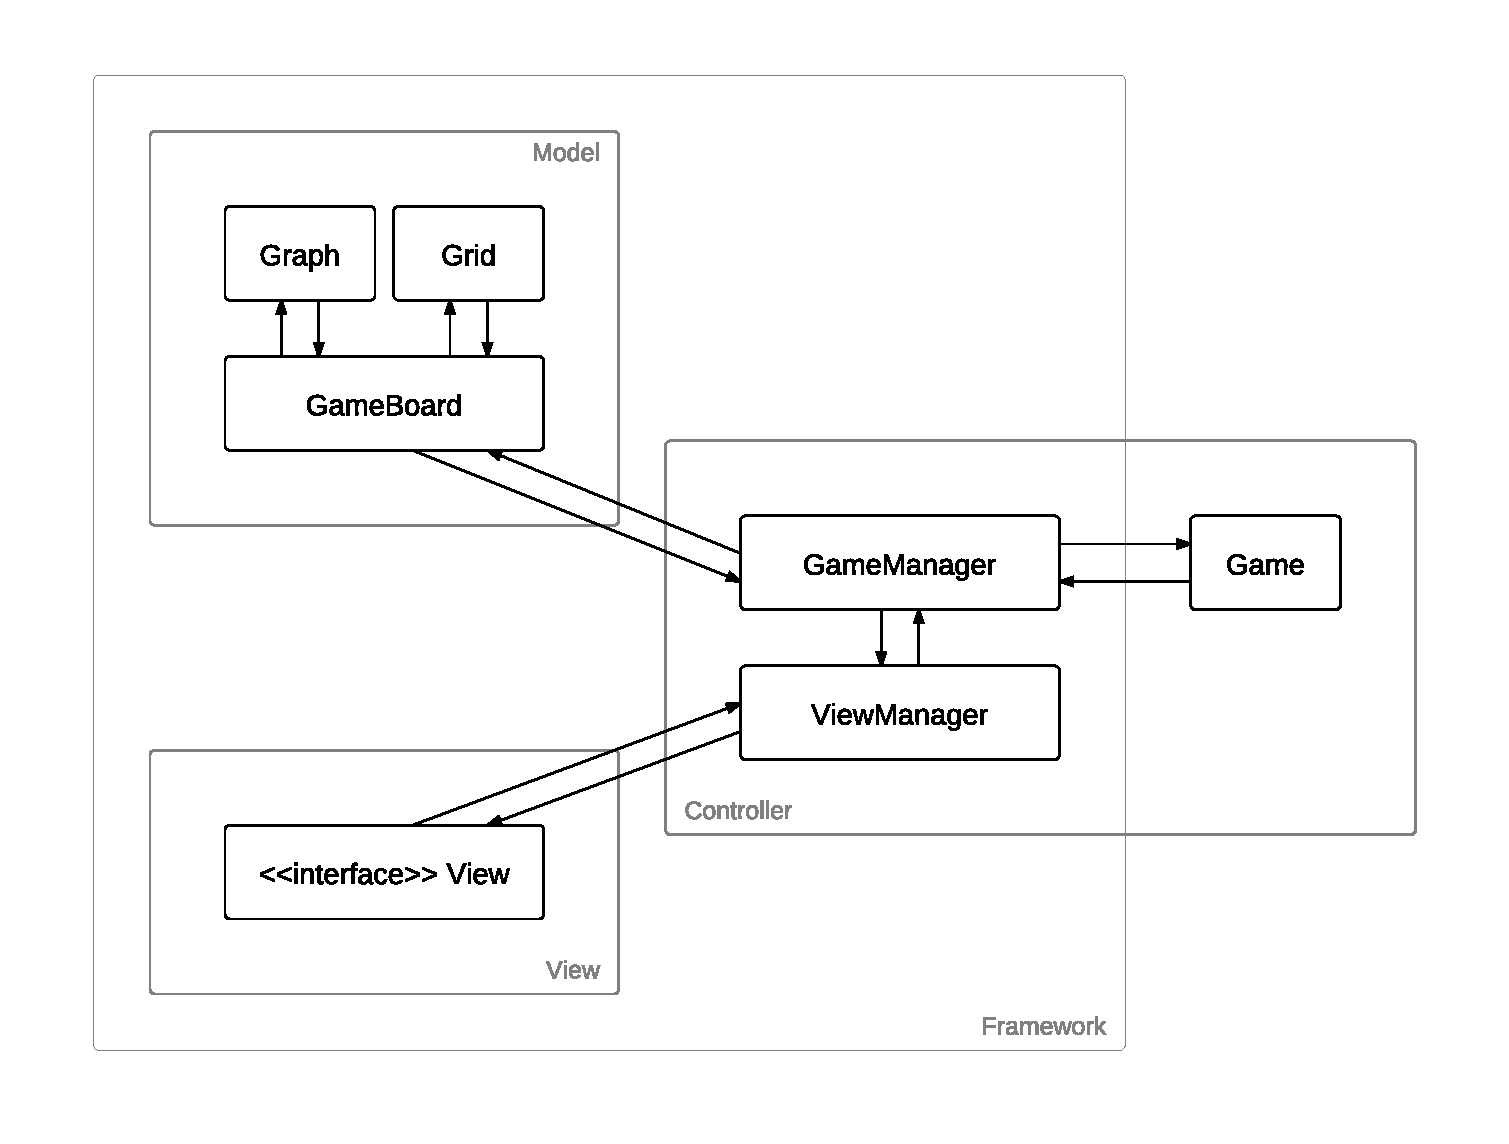
\includegraphics[width=1\textwidth]{archMVC.pdf}
	\caption{Diagram showing the realization of the \gls{MVC} design pattern by the framework.}
	\label{img:archMVC}
\end{figure}
\section{Class Diagram}

\begin{figure}[h]
	\centering
	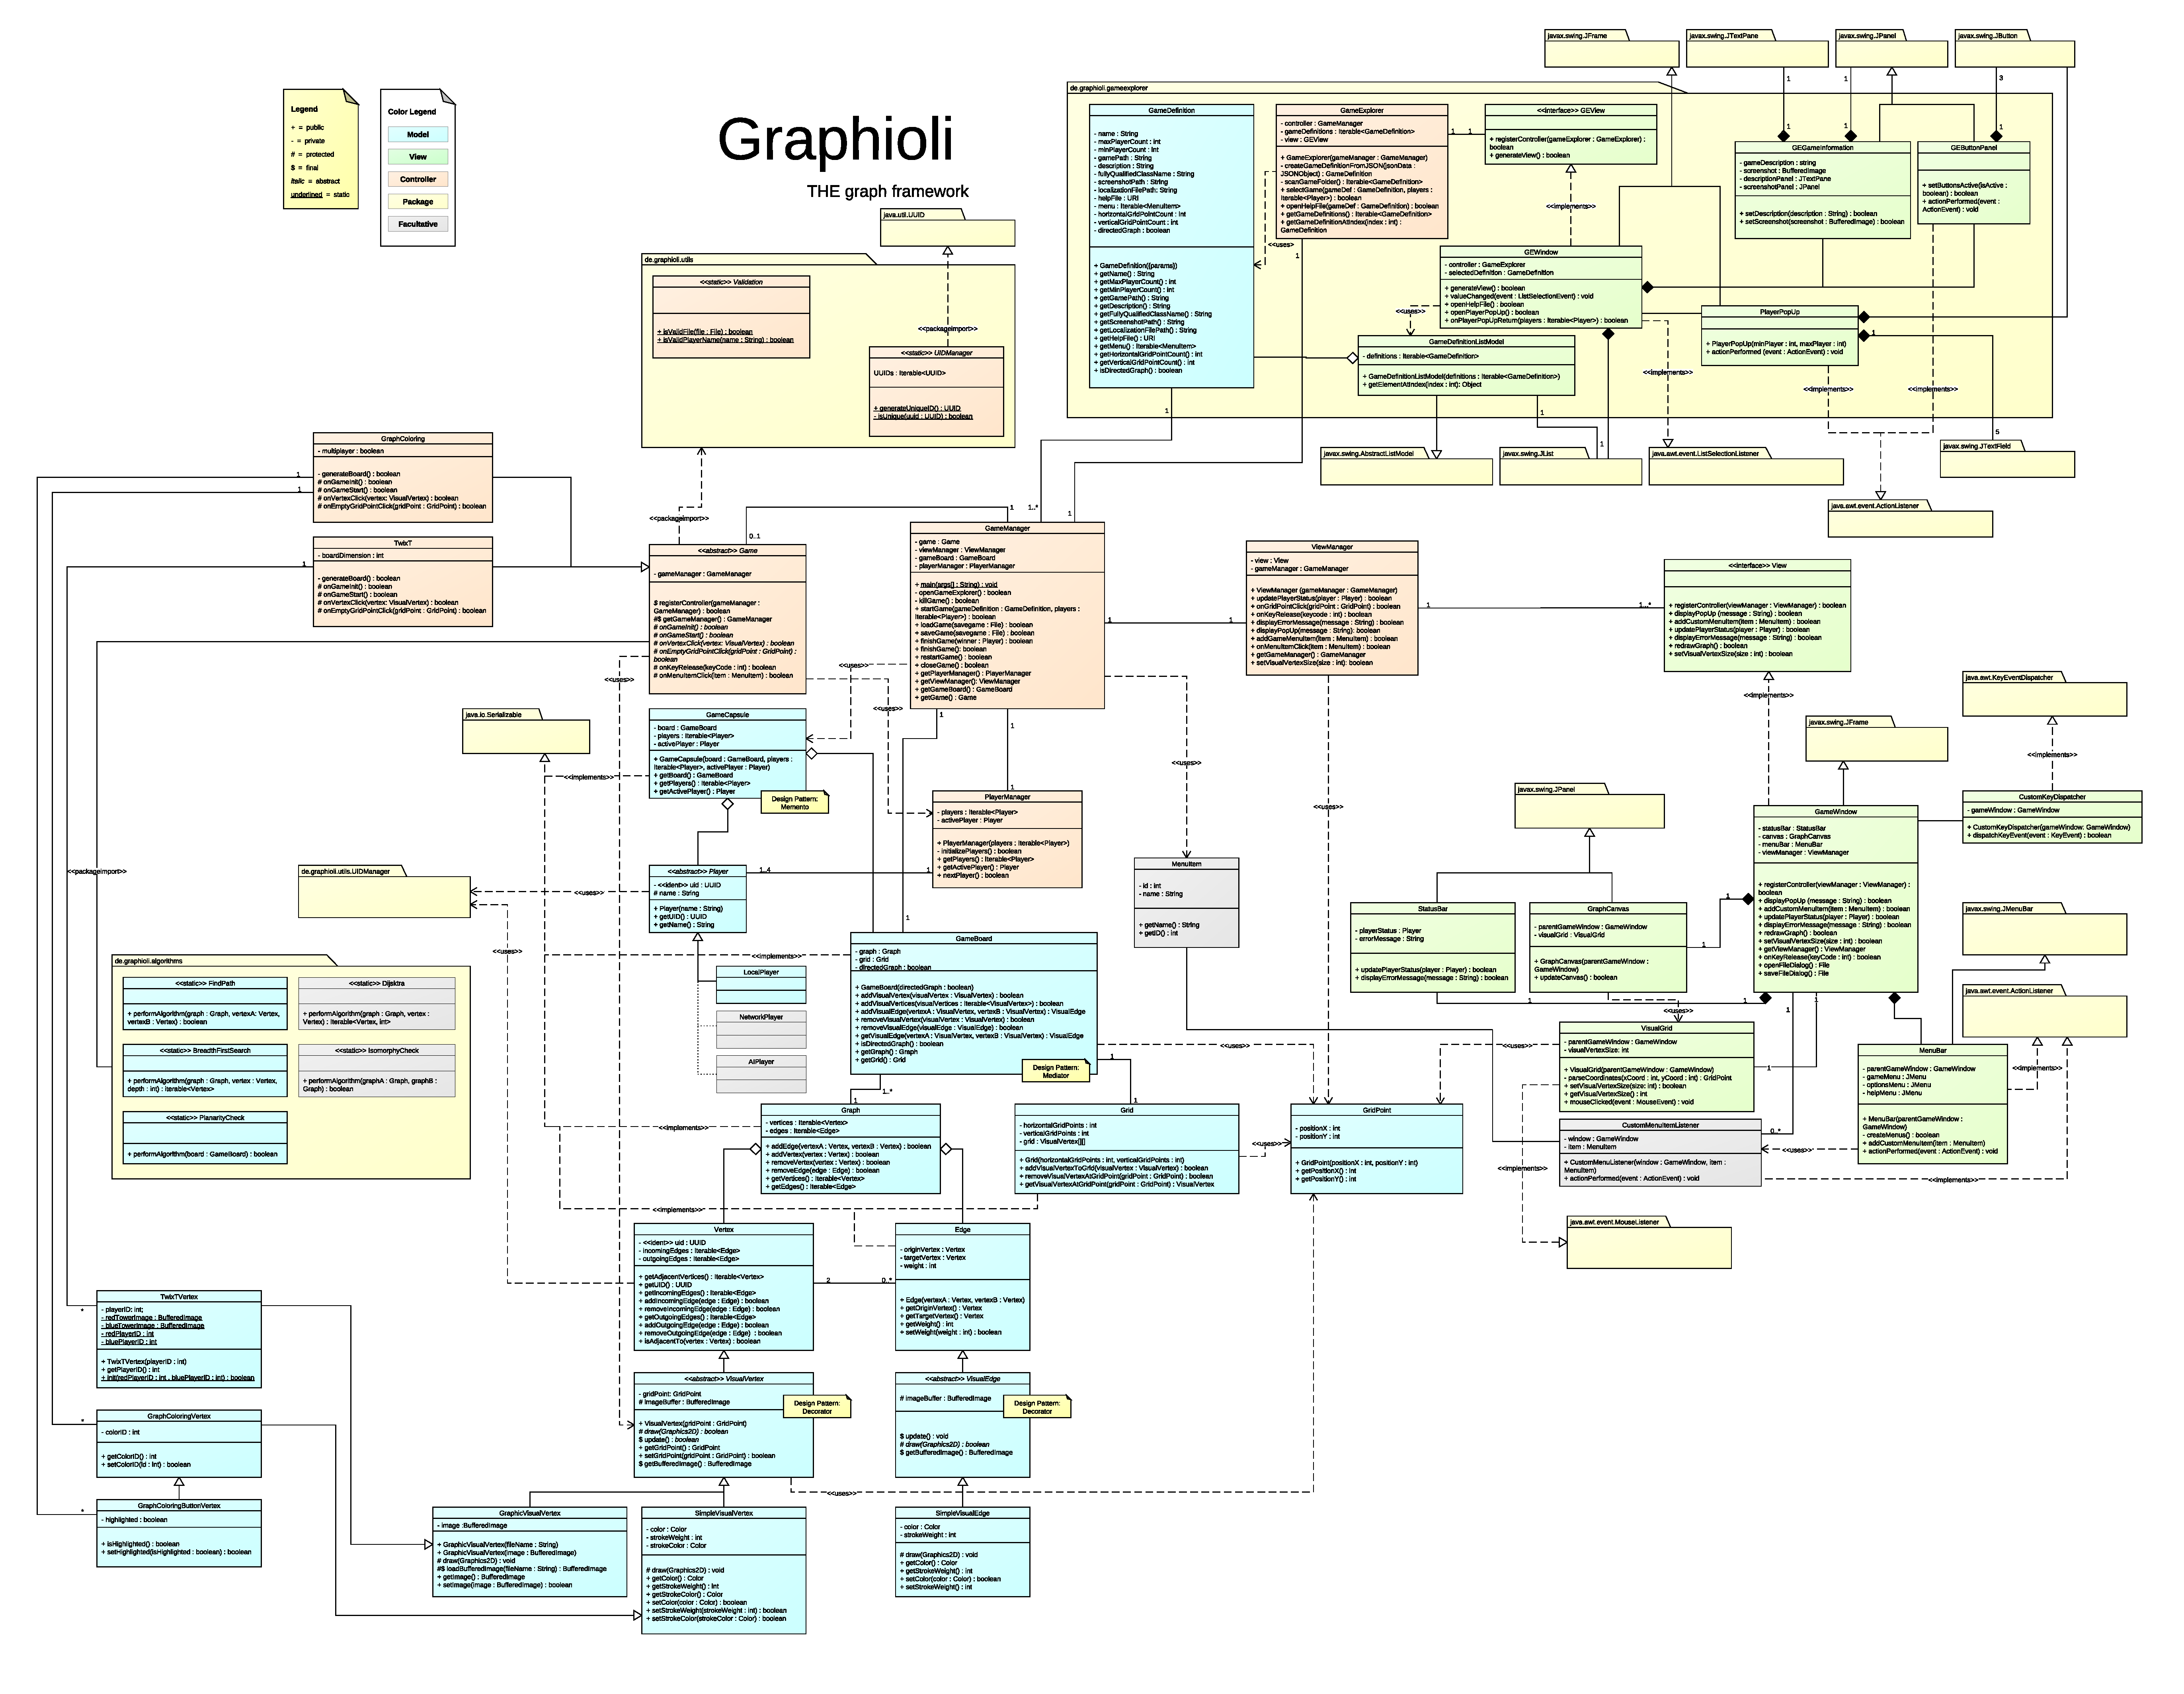
\includegraphics[angle=90,width=0.78\textwidth,keepaspectratio]{classGraphioli.pdf}
	\caption{Class diagram showing the framework's inter-class dependencies. The MVC design pattern is outlined by different colors.}
	\label{img:classGraphioli}
\end{figure}
\section{Sequence Diagrams}

\begin{figure}[h]
	\centering
	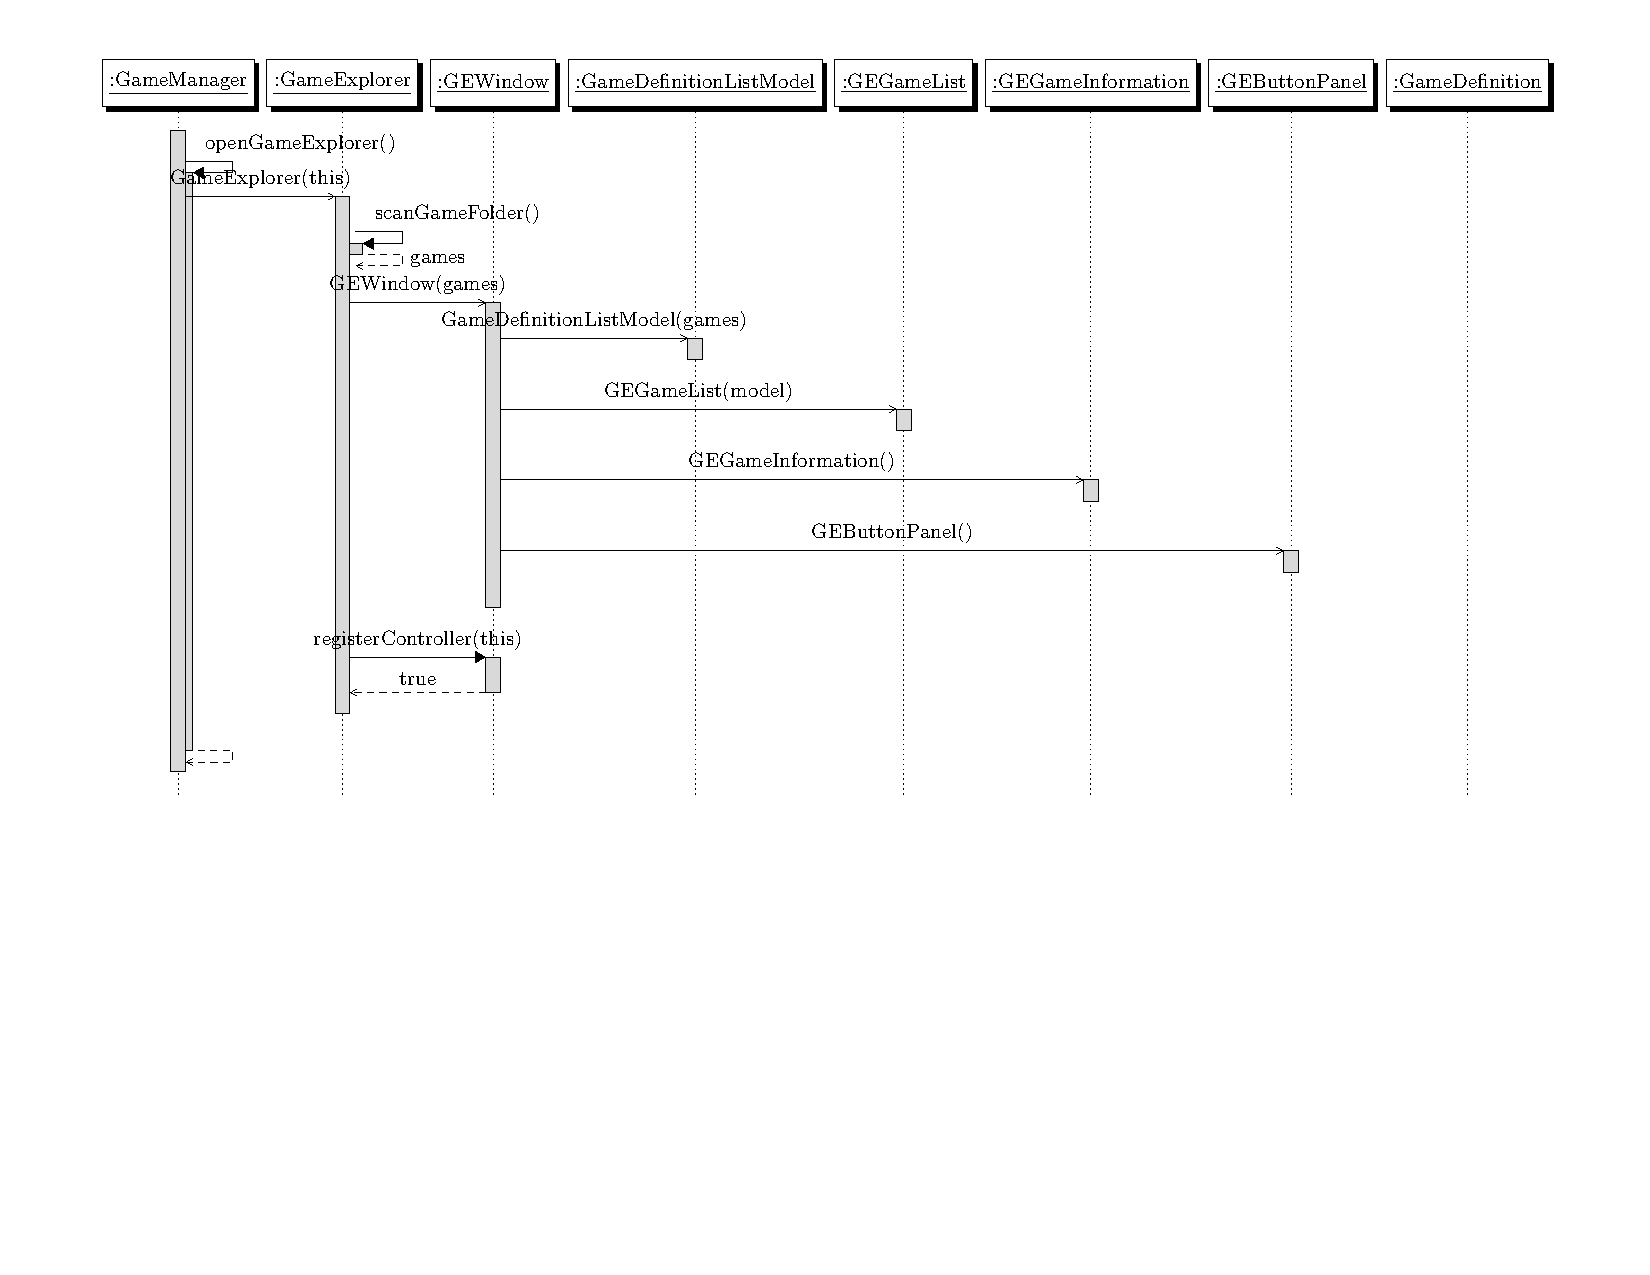
\includegraphics[page=1,angle=90,height=0.72\textheight,keepaspectratio]{seqGameExplorer.pdf}
	\caption{Sequence diagram showing the process of initializing the \gameexplorer.}
	\label{img:seqGameExplorer}
\end{figure}

\begin{figure}[h]
	\centering
	\includegraphics[page=2,angle=90,width=1\textwidth]{seqGameExplorer.pdf}
	\caption{Sequence diagram showing the process of selecting a game with an initialized \gameexplorer.}
	\label{img:seqGameExplorer}
\end{figure}

\begin{figure}[h]
	\centering
	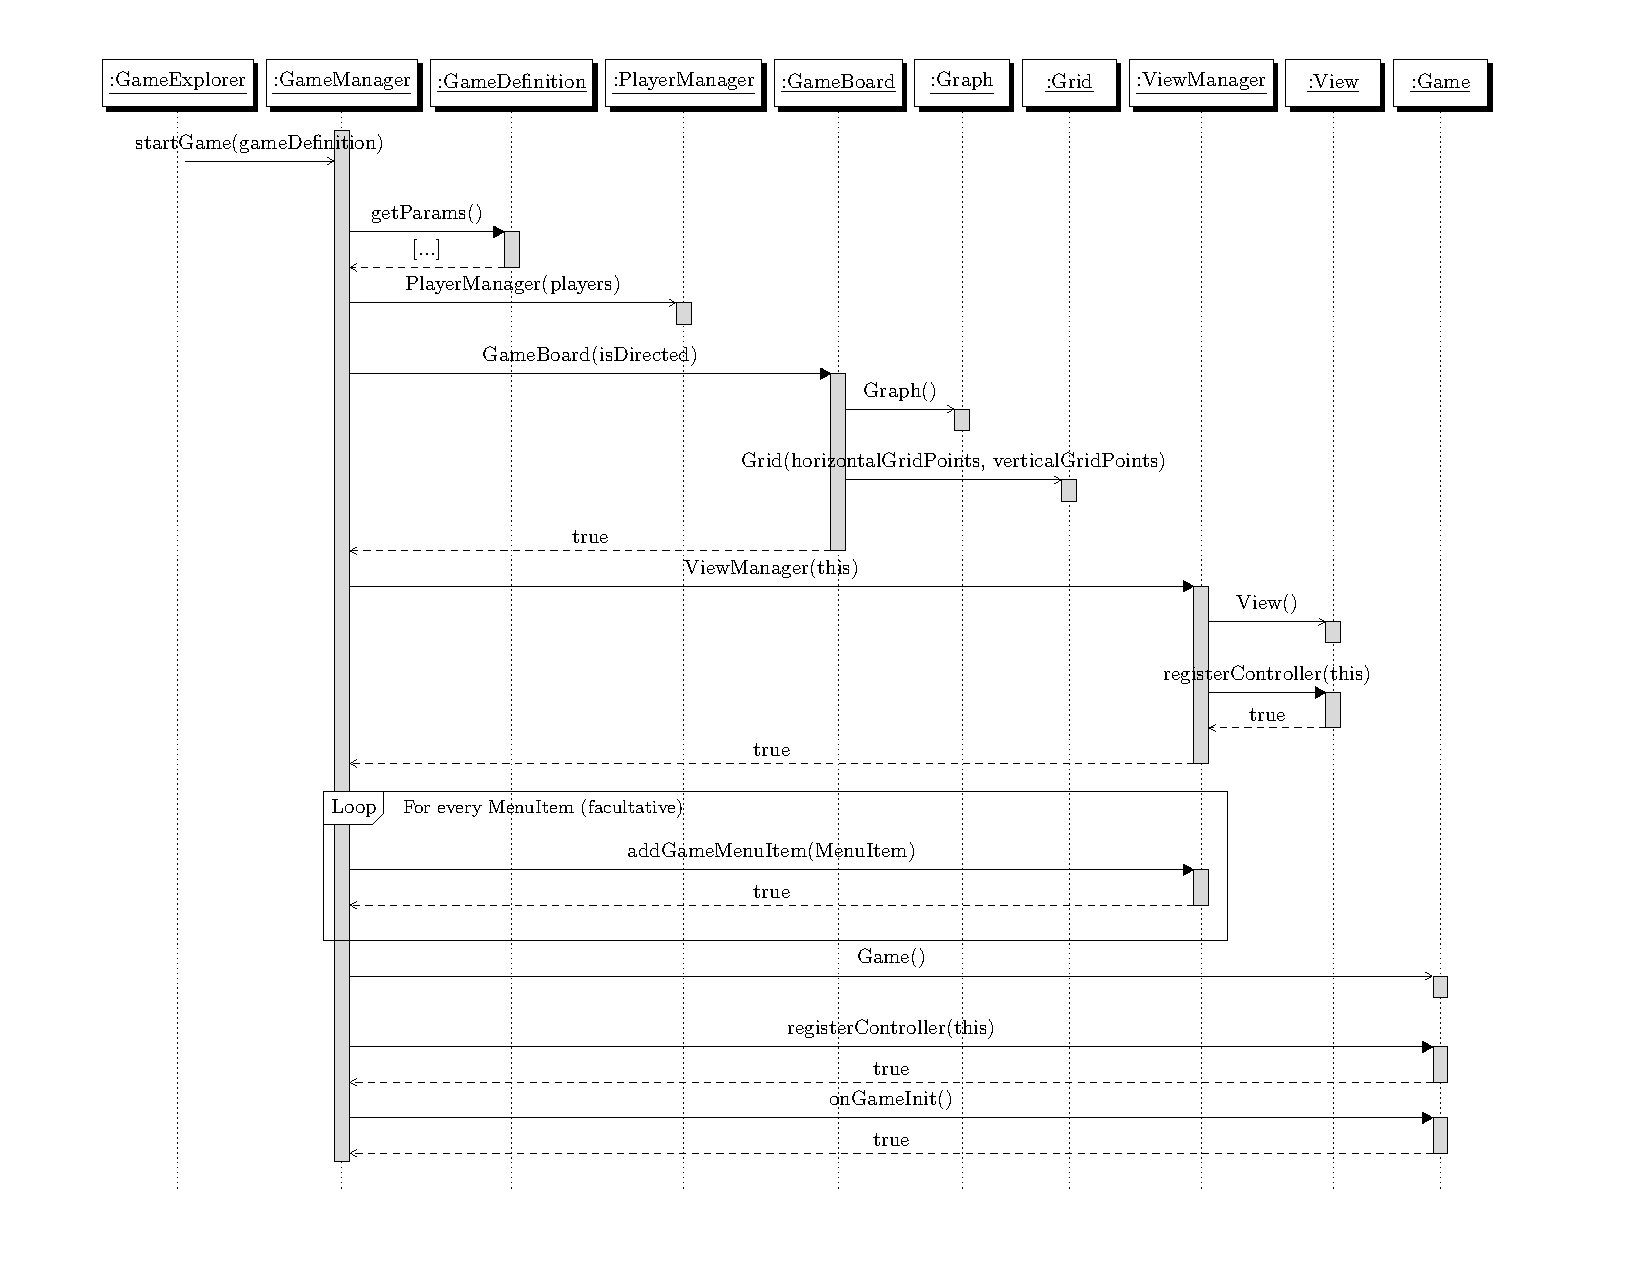
\includegraphics[angle=90,width=1\textwidth]{seqGameInitialization.pdf}
	\caption{Sequence diagram showing the process of a game's initialization.}
	\label{img:seqGameInitialization}
\end{figure}

\begin{figure}[h]
	\centering
	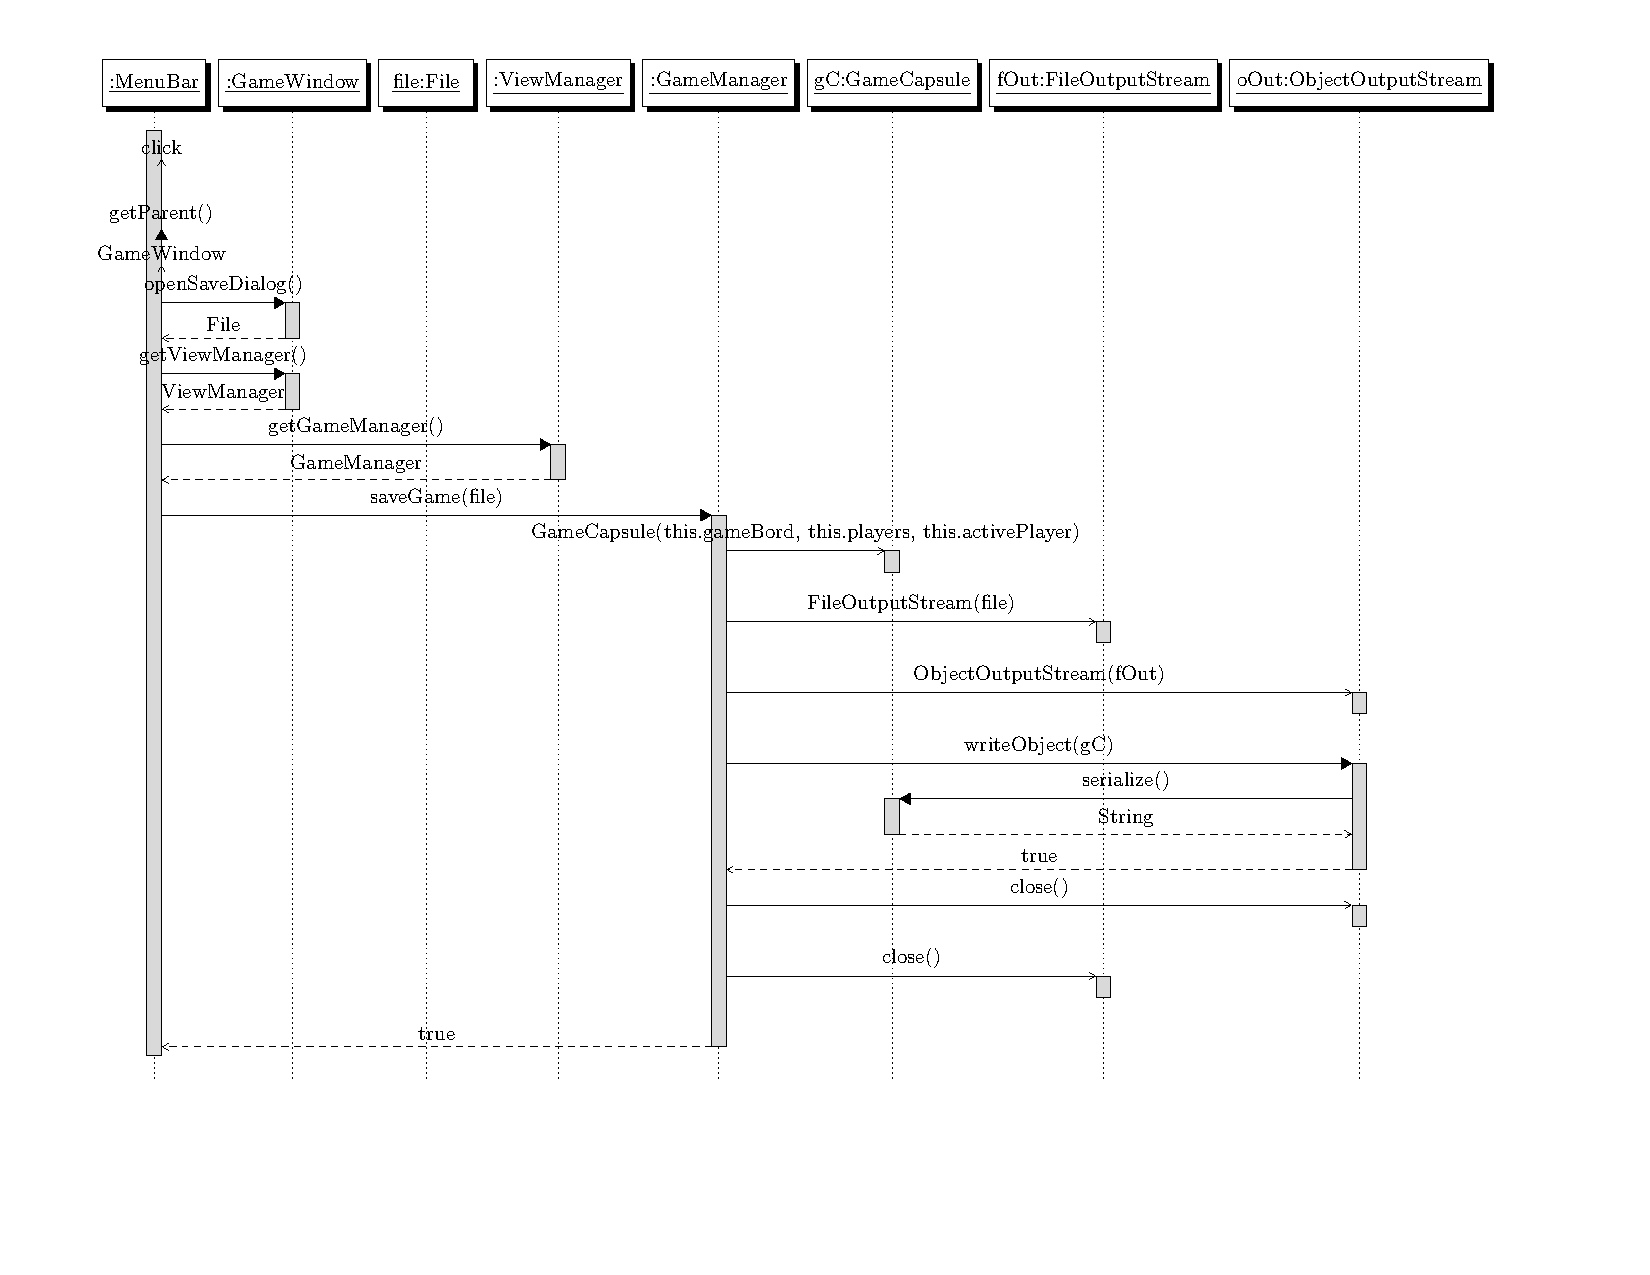
\includegraphics[page=1,angle=90,width=1\textwidth]{seqSaveLoadGame.pdf}
	\caption{Sequence diagram showing the process of saving a game.}
	\label{img:seqSaveLoadGame}
\end{figure}

\begin{figure}[h]
	\centering
	\includegraphics[page=2,angle=90,width=1\textwidth]{seqSaveLoadGame.pdf}
	\caption{Sequence diagram showing the process of loading a game.}
	\label{img:seqSaveLoadGame}
\end{figure}
\section{Miscellaneous}
\subsection{Game property file}

\begin{lstlisting}[caption=An example of a property file]
/* This is an example property file for the 'Dummy' game. */

{
    "game": [{
        "name": "Dummy",
        "gamePath": "..path/to/dummy/",
        "fullyQualifiedClassName": "de.graphioli.game.Dummy",
        "description": "This is a description for the Dummy game",
        "screenshot": "./screenshot.png",
        "languageFile": "./language_en.txt",
        "helpFile": "../helpFile.pdf",
        "maxPlayerCount": 1,
        "minPlayerCount": 4,
        "menuItem": [{
            "save": 1,
            "load": 2,
            "exit": 3
        }],
        "horizontalGridPointCount": 100,
        "verticalGridPointCount": 100
    }]
}
\end{lstlisting}

\section{Glossary}

\end{document}
